\documentclass{article}
\usepackage{tikz}
\usetikzlibrary{arrows.meta}

\begin{document}

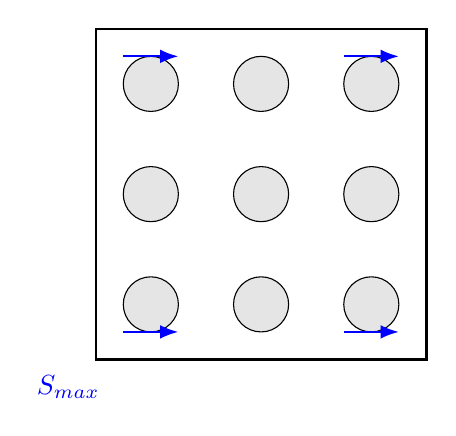
\begin{tikzpicture}[scale=0.7]
    % Define the grid
    \draw[thick] (-1,-1) -- (5,-1) -- (5,5) -- (-1,5) -- cycle;
    % Draw the Seifert circles
    \draw[fill=gray!20] (0,0) circle (0.5);
    \draw[fill=gray!20] (4,0) circle (0.5);
    \draw[fill=gray!20] (0,4) circle (0.5);
    \draw[fill=gray!20] (4,4) circle (0.5);
    \draw[fill=gray!20] (2,2) circle (0.5);
    \draw[fill=gray!20] (2,0) circle (0.5);
    \draw[fill=gray!20] (2,4) circle (0.5);
    \draw[fill=gray!20] (0,2) circle (0.5);
    \draw[fill=gray!20] (4,2) circle (0.5);
    % Draw the arrows indicating orientation
    \draw[-Latex, thick, blue] (3.5,4.5) -- (4.5,4.5);
    \draw[-Latex, thick, blue] (-0.5,-0.5) -- (0.5,-0.5);
    \draw[-Latex, thick, blue] (3.5,-0.5) -- (4.5,-0.5);
    \draw[-Latex, thick, blue] (-0.5,4.5) -- (0.5,4.5);
    % Label the grid diagram
    \node at (-1.5, -1.5) {\textcolor{blue}{\(S_{\text{max}}\)}};
\end{tikzpicture}

\end{document}